\documentclass[12pt]{article}
\usepackage{amsmath}
\usepackage{amsfonts}
\usepackage{amssymb}
\usepackage{graphicx}
\usepackage[a4paper, margin=0.98in]{geometry}
\usepackage{physics}
\usepackage{float}
\usepackage{booktabs}
\usepackage{makecell}
\usepackage{helvet}
\usepackage{fancyhdr}
\usepackage{titling}
\usepackage{longtable}
\usepackage{caption}
\usepackage{enumitem}
\usepackage{circuitikz}
\usepackage[hidelinks]{hyperref}

% Define header
\pagestyle{fancy}
\fancyhf{}
\fancyhead[R]{PH3204: Electronics Laboratory}

% Title
\title{
  \vspace{-2cm}
  \Huge \textbf{PH3204: Electronics Laboratory} \\[0.4cm]
  \Large \textit{Experiment 01: Study of Zener Diode as a Voltage Regulator and Use of IC 7805 Voltage Stabilizer}
}

\author{
  \textbf{Ronit Bhuyan (22MS025)} \\[0.2cm]
  \textbf{Sub-Group B01}
}

\date{}

\begin{document}

\maketitle

\tableofcontents
\noindent\rule{\textwidth}{0.4pt}
\newpage

\section{Theory}
\subsection{Zener Diode as Voltage Regulator}
Zener Diode is a heavily doped p-n junation diode which is designed to operate in reverse bias. When operated in reverse bias , if the voltage across the diode exceeds the zener breakdown voltage $V_Z$, the diode enters the \textit{zener breakdown region} where voltage across the diode remains constant irrespective of the current flowing through it. \\
This property of the zener diode is exploited for Voltage Regulation. The circuit diagram of a zener diode used as a voltage regulator has been shown below.
\begin{figure}[H]
    \centering
    \begin{circuitikz}[american voltages]
        % Zener Diode with coloring
        \draw
        (5,-1) to [zzD] (5,2)
        % Current meter and upper connections
        to [rmeter, t=mA, l_=$i_z$] (5, 3)
        to [short, -*] (5, 4)
        to [rmeter, t=mA, l_=$i_s$] (2, 4)
        to [R, l^=$R_s$] (1, 4)
        to [short] (0, 4)
        % Battery connection
        to [battery, l=$V_{\mathrm{i}}$] (0, -1)
        to [short] (0, -1)
        to [short] (5, -1)
        % Load branch
        (5, 4) to [short] (7, 4)
        to [R, l=$R_C$] (7, 2)
        to [rmeter, t=mA, l_=$i_L$] (7, 1)
        to [vR, l=$R_{\mathrm{L}}$] (7, -1)
        to [short] (5, -1)
        % Probing points
        (7, 4) to [short, -*] (8.5, 4)
        (7, -1) to [short, -*] (8.5, -1);
		%ground
		\draw (5,-1) node[ground]{};
		\draw (8.5,-1) to [rmeter, t=v, l_=$V_{\mathrm{out}}$] (8.5,4);
    \end{circuitikz}
    \caption{Circuit Diagram for Zener Diode as a Voltage Regulator}
\end{figure}\noindent
\subsubsection*{Line Regulation}

Line regulation corresponds to the ability of keeping the output voltage constant despite changes in the input voltage. It is defined as the change in output volatge for a unit change in input voltage.\\
To measure this we remove the resistor $(R_L)$ and keep the resistor $(R_L)$ fixed. We then vary the input voltage $V_{i}$ in regular intervals and measure the output voltage $V_{out}$. When the input volatge goes beyond the breakdown voltage, the output voltage $V_{out}$ remains constant at $V_Z$. The current through the resistor $R_L$ therefoee becomes constant.
\begin{equation*}
	\delta i_s= \delta i_z
\end{equation*}

\subsubsection*{Load Regulation}
Load regulation corresponds to the ability of keeping the output voltage constant despite changes in the load resistance. It is defined as the change in output voltage for a unit change in load resistance. When the load resistance goes beyond a threshold value, the output voltage $V_{out}$ remains constant. The current through the load resistor therefore becomes constant. Thus, 
\begin{equation*}
	\delta i_z= -\delta i_L
\end{equation*}
\subsection{Voltage Regulator IC7805}
As mentioned in the above section, a zener diode can be used as a volatge regulator. But, usually the output voltage doesn't remain completely stable and there is a small variation in the output voltage. To overcome this, we use a voltage regulator IC. The IC 7805 is a voltage regulator IC which provides a stable output voltage of $5V$. The circuit diagram for using IC 7805 as a voltage regulator has been shown below.

\begin{figure}[H]
	\centering
	\begin{circuitikz}[american voltages]
		\draw
		(-1,0) -- (1,0)
		++(1,0) node[rectangle,draw,fill=white,
		minimum width=3.1cm,minimum height=1.25cm,
		label={[below]north:{\small \fbox{IC7805}}},
		label={[right]west:{\small In}},
		label={[above]south:{\small GND}},
		label={[left]east:{\small Out}}]{}
		(2,-0.6) -- (2,-5)
		(3,0) -- (5,0)
		to [short, -] (5.3,0)
		(5.3,0) to [short, -] (7.5,0) % Junction point just above Rc
		(5.3,0) to [short] (5.3,-0.3) to [R=$R_c$] (5.3,-1.5)
		to [rmeter, t=mA, l=$i_L$, i=${}$] (5.3,-2.9)
		to [vR, l=$R_{\mathrm{L}}$] (5.3,-5)
		to [short] (-1,-5);
		\draw (-1, -1) to [battery, l_=$V_{\mathrm{i}}$] (-1,-5);
		\draw (-1, -1) to [short] (-1,0)
		(5.3,-5) to [short, -] (7.5, -5);
		\node at (4.3,-5) [ground]{};
		\draw (7.5,0) to [rmeter, t=V, l=$V_{\mathrm{out}}$, *-*] (7.5,-5);
	\end{circuitikz}
	\caption{Circuit Diagram for regulation using IC 7805}
	\label{fig:theory_02}
\end{figure}\noindent

\section{Zener Diode as a voltage Regulator}
\subsection{Line Regulation}

To study the line regulation property of zener diode, we keep the resistance $R_C$ fixed at $2.2k\Omega$. We then vary the input voltage $V_i$ in regular intervals and measure the output voltage $V_{out}$, the current through the diode, $I_{z}$ and through the series resistance ,$I_S$. The data has been tabulated below


\begin{longtable}{|l|l|l|l|}
	\hline
  $V_\mathrm{i}$ (V) & $I_\mathrm{s}$ (mA) & $V_\mathrm{out}$ (v) & $I_\mathrm{z}$ (mA) \\ \hline
	\endfirsthead
	\hline
	$V_i$ (V) & $I_s$ (mA) & $V_{out}$ (V) & $I_z$ (mA) \\ \hline
	\endhead
	\hline
	\endfoot
	\hline
	\endlastfoot
    0                 & 0                 & 0                  & 0                 \\ \hline
    0.53              & 0.12              & 0.27               & 0                 \\ \hline
    1.02              & 0.23              & 0.51               & 0                 \\ \hline
    1.5               & 0.35              & 0.77               & 0                 \\ \hline
    2                 & 0.46              & 1.01               & 0                 \\ \hline
    2.51              & 0.58              & 1.27               & 0                 \\ \hline
    2.98              & 0.69              & 1.51               & 0                 \\ \hline
    3.5               & 0.81              & 1.77               & 0                 \\ \hline
    4.01              & 0.93              & 2.03               & 0                 \\ \hline
    4.51              & 1.05              & 2.28               & 0                 \\ \hline
    5.09              & 1.18              & 2.58               & 0                 \\ \hline
    5.49              & 1.27              & 2.78               & 0.0002            \\ \hline
    6.02              & 1.39              & 3.03               & 0.0008            \\ \hline
    6.49              & 1.51              & 3.28               & 0.0023            \\ \hline
    7                 & 1.63              & 3.54               & 0.004             \\ \hline
    7.49              & 1.74              & 3.78               & 0.0083            \\ \hline
    7.99              & 1.86              & 4.03               & 0.0161            \\ \hline
    8.52              & 1.98              & 4.29               & 0.0337            \\ \hline
    9.02              & 2.11              & 4.54               & 0.0637            \\ \hline
    9.5               & 2.22              & 4.77               & 0.1132            \\ \hline
    9.98              & 2.34              & 4.99               & 0.1666            \\ \hline
    10.51             & 2.48              & 5.16               & 0.2               \\ \hline
    10.98             & 2.68              & 5.29               & 0.25              \\ \hline
    11.45             & 2.85              & 5.39               & 0.3               \\ \hline
    12                & 3.07              & 5.46               & 0.6               \\ \hline
    12.5              & 3.28              & 5.51               & 0.7               \\ \hline
    12.95             & 3.47              & 5.54               & 0.9               \\ \hline
    13.46             & 3.7               & 5.57               & 1.1               \\ \hline
    14.06             & 3.97              & 5.59               & 1.4               \\ \hline
    14.49             & 4.17              & 5.61               & 1.5               \\ \hline
    14.96             & 4.38              & 5.63               & 1.8               \\ \hline
\end{longtable}\noindent

\begin{figure}[H]  
  \centering  
  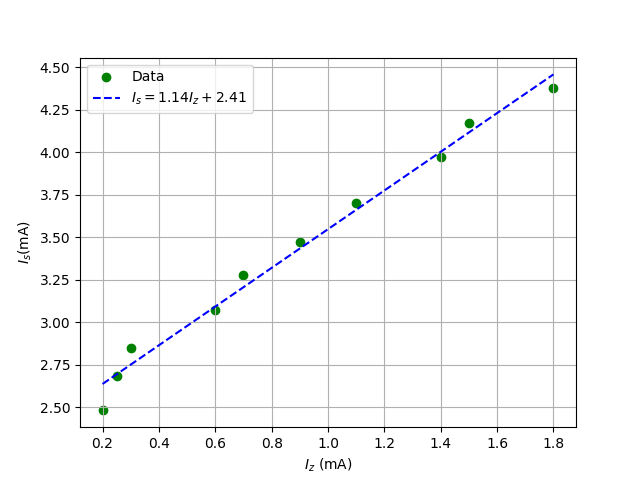
\includegraphics[width=0.8\textwidth]{D:/ronit/IISER-K/6 SEM/PH3204/Reports/exp01/part01_01.png}  % Path to your image file
  \caption{Plot of $I_z$ v/s $I_s$}  % Optional caption
  \label{fig:part01_01}  % Optional label for referencing
\end{figure}\noindent
We plot a graph between $I_z$ and $I_s$. Upon fitting the curve with a straight line we get the following fit curve.
\begin{equation*}
	I_s = 1.14I_z + 2.41
\end{equation*}
The slope of the grpah is found to be $1.14 \pm 0.002$V which verifies the fact that $\delta I_s=\delta I_z$ 
\newpage
\noindent
To estimate the breakdown voltage $V_Z$ we plot a graph between $V_{out}$ and $V_{i}$. In the graph plotted below it is clear that when the input voltage $V_i$ crosses $10.51 V$, the output voltage $V_{out}$ remains almost constant,indicating that breakdown has occured. The breakdown voltage is estimated to be $5.59 V$.
\begin{figure}[H]  
	\centering  
	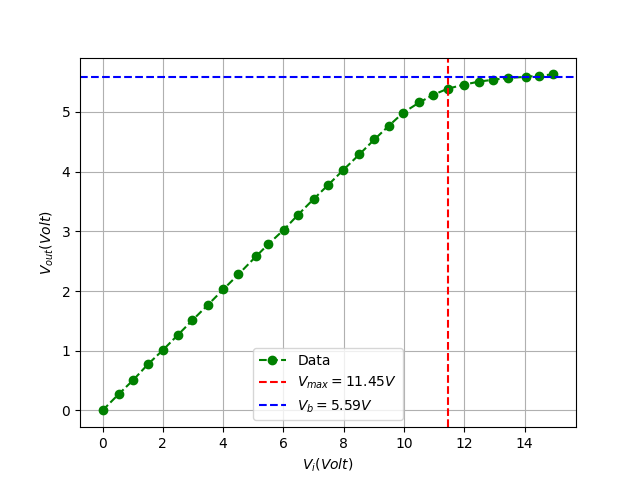
\includegraphics[width=0.8\textwidth]{D:/ronit/IISER-K/6 SEM/PH3204/Reports/exp01/part01_02.png}  % Path to your image file
	\caption{Plot of $V_{i}$ v/s $V_{out}$ to estimate the breakdown volatge}  % Optional caption
	\label{fig:part01_01}  % Optional label for referencing
  \end{figure}\noindent
\\
Note that the following part of the experiment was done on Day 2 with a different zener diode with a different breakdown voltage. 

\subsection{Load Regulation}
In this part of the experiment we keep the input voltage $V_i$ fixed at $14.6 V$. The load resistance $R_L$ is varies from $1k\Omega$ to $10k\Omega$ in regular intervals. The output voltage $V_{out}$, the current through the diode, $I_{z}$ and through the load resistance ,$I_L$ are measured. The data has been tabulated below.\\
The data has been taken twice, once without the current limiting resistor $R_C$ and once with it.\\
\\
\textbf{Without current limiting resistor $R_C$}
\begin{longtable}{|c|c|c|c|}
    \hline
    $R_{L}$ ($\Omega$) & $i_{L}$ (mA) & $i_{Z}$ (mA) & $V_{out}$ (V) \\ 
    \hline
    \endfirsthead
    \hline
    \textbf{$R_{L}$ ($\Omega$)} & \textbf{$i_{L}$ (mA)} & \textbf{$i_{Z}$ (mA)} & \textbf{$V_{out}$ (V)} \\ 
    \hline
    \endhead

    \hline
    \endfoot
    \endlastfoot

    % TABLE DATA
    1.2                     & 6.9               & 0                 & 0.0108             \\ \hline
    48.2                    & 6.6               & 0                 & 0.32               \\ \hline
    99.1                    & 6.4               & 0                 & 0.797              \\ \hline
    151.4                   & 6.2               & 0                 & 1.111              \\ \hline
    213                     & 6.2               & 0                 & 1.389              \\ \hline
    278                     & 6                 & 0                 & 1.678              \\ \hline
    303                     & 5.9               & 0                 & 1.876              \\ \hline
    359                     & 5.8               & 0                 & 2.1                \\ \hline
    403                     & 5.7               & 0                 & 2.31               \\ \hline
    452                     & 5.4               & 0                 & 2.92               \\ \hline
    502                     & 5.5               & 0                 & 2.77               \\ \hline
    556                     & 5.4               & 0                 & 3.01               \\ \hline
    603                     & 5.2               & 0                 & 3.16               \\ \hline
    655                     & 5.3               & 0                 & 3.26               \\ \hline
    697                     & 5.1               & 0                 & 3.55               \\ \hline
    751                     & 5                 & 0                 & 3.78               \\ \hline
    806                     & 4.9               & 0                 & 3.95               \\ \hline
    859                     & 4.8               & 0                 & 4.15               \\ \hline
    902                     & 4.8               & 0                 & 4.29               \\ \hline
    955                     & 4.6               & 0                 & 4.61               \\ \hline
    1007                    & 4.6               & 0                 & 4.64               \\ \hline
\end{longtable}\noindent
From the above table, we see that the maximum output voltage reached without using $R_C$ is $V_{out} =4.64 V$ which is less than the output voltage obtained after reaching the breakdown voltage $(6.55 V)$ calculated from the previous part, indicating that the breakdown has not been reached, which is why we are getting negligible current.\\
\\
\textbf{With current limiting resistor $R_C$}
\begin{longtable}{|c|c|c|c|}
    \hline
    $R_\text{L}$ ($\Omega$) & $i_\text{L}$ (mA) & $i_\text{Z}$ (mA) & $V_\text{out}$ (V) \\ 
    \hline
    \endfirsthead
    \hline
    $R_\text{L}$ ($\Omega$) & $i_\text{L}$ (mA) & $i_\text{Z}$ (mA) & $V_\text{out}$ (V) \\ 
    \hline
    \endhead

    \endfoot

    
    1.3                     & 3                 & 0.8               & 6.54               \\ \hline
    50.7                    & 2.9               & 0.8               & 6.54               \\ \hline
    101.5                   & 2.8               & 0.9               & 6.54               \\ \hline
    151                     & 2.8               & 0.9               & 6.54               \\ \hline
    203                     & 2.7               & 1                 & 6.54               \\ \hline
    258                     & 2.7               & 1                 & 6.54               \\ \hline
    303                     & 2.6               & 1.1               & 6.54               \\ \hline
    360                     & 2.5               & 1.2               & 6.54               \\ \hline
    405                     & 2.5               & 1.2               & 6.54               \\ \hline
    452                     & 2.5               & 1.2               & 6.54               \\ \hline
    505                     & 2.4               & 1.3               & 6.54               \\ \hline
    556                     & 2.4               & 1.3               & 6.54               \\ \hline
    604                     & 2.3               & 1.4               & 6.54               \\ \hline
    646                     & 2.3               & 1.4               & 6.54               \\ \hline
    701                     & 2.3               & 1.4               & 6.54               \\ \hline
    755                     & 2.2               & 1.5               & 6.54               \\ \hline
    798                     & 2.2               & 1.5               & 6.54               \\ \hline
    858                     & 2.1               & 1.6               & 6.54               \\ \hline
    907                     & 2.1               & 1.6               & 6.54               \\ \hline
    951                     & 2.1               & 1.6               & 6.54               \\ \hline
    1010                    & 2                 & 1.7               & 6.54               \\ \hline

\end{longtable}
\noindent
We plot a graph between $I_z$ and $I_L$. Upon fitting the curve with a straight line we get the following fit curve.
\begin{equation*}
	I_L = -1.00I_z + 3.70
\end{equation*}
\begin{figure}[H]  
	\centering  
	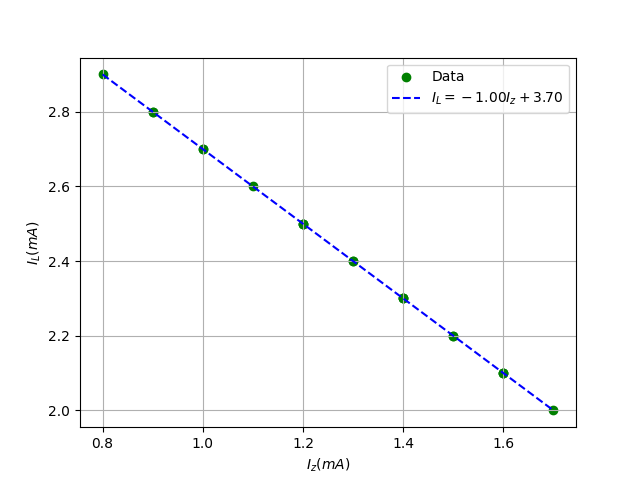
\includegraphics[width=0.8\textwidth]{D:/ronit/IISER-K/6 SEM/PH3204/Reports/exp01/part01_03.png}  % Path to your image file
	\caption{Plot of $I_z$ v/s $I_L$ with constant $V_i$=14.6V}  % Optional caption
	\label{fig:part01_01}  % Optional label for referencing
  \end{figure}
  \begin{figure}[H]  
	\centering  
	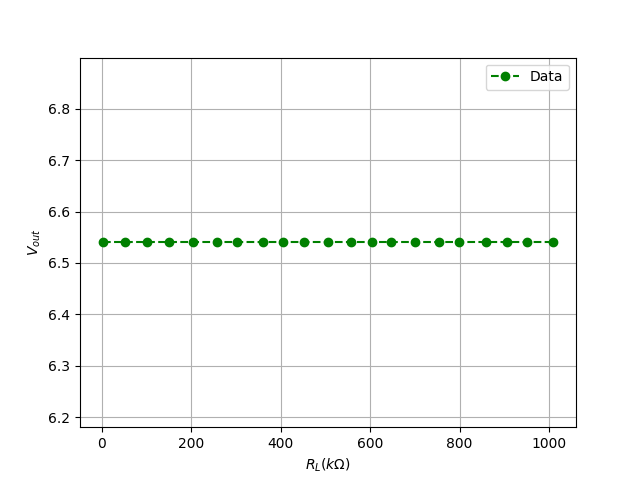
\includegraphics[width=0.8\textwidth]{D:/ronit/IISER-K/6 SEM/PH3204/Reports/exp01/part01_04_update.png}  % Path to your image file
	\caption{Plot of $R_L$ v/s $V_{out}$ with constant $V_i$=14.6V}  % Optional caption
	\label{fig:part01_01}  % Optional label for referencing
  \end{figure}\noindent
From the graph plotted above we could verfiy that the breakdown voltage of the zener diode is $6.54 V$.
\section{IC7805 as a Voltage Regulator}
\subsection{Line Regulation}
In line regulation, we have used current limiting resistor $R_C=2.2 k\Omega$ and have removed the resistance $R_L$.The input voltage $V_i$ is varied from $0 V$ to $10V$ in regular intervals and the output voltage $V_{out}$ is measured. The data has been tabulated below.
\begin{longtable}{|c|c|c|}
	\hline
   {$\mathrm{V_{i} (V)}$} & $\mathrm{I_L (mA)}$ & $\mathrm{V_{out} (V)}$ \\ \hline
	\endfirsthead
	
	\hline
	{$\mathrm{V_{i} (V)}$} & $\mathrm{I_L (mA)}$ & $\mathrm{V_{out} (V)}$ 
	\endhead
	
	\hline
	\endfoot
	
	\hline
	\endlastfoot
		0.04              & 0                 & 0.01               \\ \hline
		0.51              & 0                 & 0.01               \\ \hline
		1.01              & 0                 & 0.01               \\ \hline
		1.51              & 0                 & 0.1                \\ \hline
		2                 & 0.59              & 1.26               \\ \hline
		2.5               & 0.81              & 1.71               \\ \hline
		2.99              & 1.02              & 2.17               \\ \hline
		3.5               & 1.25              & 2.63               \\ \hline
		4.01              & 1.46              & 3.09               \\ \hline
		4.51              & 1.69              & 3.56               \\ \hline
		5                 & 1.9               & 4.01               \\ \hline
		5.51              & 2.12              & 4.47               \\ \hline
		6.04              & 2.36              & 4.96               \\ \hline
		6.45              & 2.37              & 4.99               \\ \hline
		7                 & 2.37              & 4.99               \\ \hline
		7.54              & 2.37              & 4.99               \\ \hline
		8.03              & 2.37              & 4.99               \\ \hline
		8.55              & 2.37              & 4.99               \\ \hline
		9.05              & 2.37              & 4.99               \\ \hline
		9.47              & 2.37              & 4.99               \\ \hline
		10.01             & 2.37              & 4.99               \\ \hline
\end{longtable}\noindent
In the graph plotted in the next page, we see that after the input voltage crosses $6.04$V the output volatge remains constant at $4.99V (\approx 5V)$, which is what we had expected. 
\begin{figure}[H]  
	\centering  
	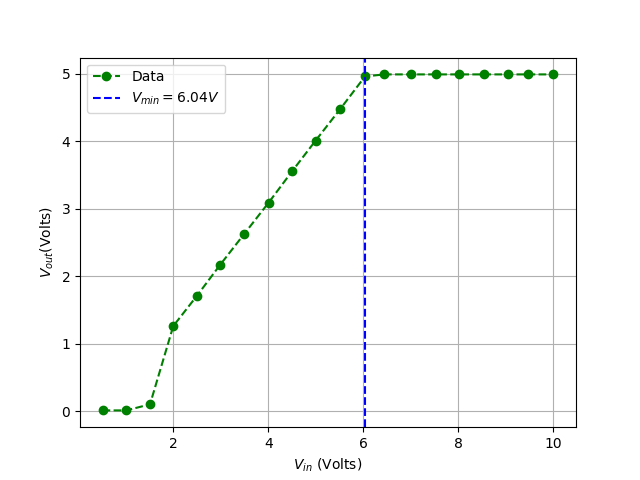
\includegraphics[width=0.8\textwidth]{D:/ronit/IISER-K/6 SEM/PH3204/Reports/exp01/part02_01.png}  % Path to your image file
	\caption{Plot depicting $V_{i}$ v/s $V_{out}$}  % Optional caption
	\label{fig:part01_01}  % Optional label for referencing
  \end{figure}
\subsection{Load Regulation}
For load regulation, we have kept the input voltage $V_i$ at 14.6 V, and while the resistor $R_L$ is varied from $0 k\Omega$ to $10 k\Omega$ in regular intervals. The output voltage $V_{out}$ is measured. The data recorded has been tabled below.
\begin{longtable}{|c|c|c|}
	\hline
	${R_L}$ (${\Omega}$ & ${i_L}$ (mA) & ${V_0}$ (V) \\ \hline
	\endfirsthead
	
	\hline
	${R_L}({\Omega})$ & ${i_L}$ (mA) & ${V_0}$ (V) \\ \hline
	\endhead
	
	\hline
	\endfoot
	
	\hline
	\endlastfoot
		1.1                     & 2.38              & 5                  \\ \hline
		50.6                    & 2.32              & 5                  \\ \hline
		100.2                   & 2.27              & 5                  \\ \hline
		149.6                   & 2.22              & 5                  \\ \hline
		205                     & 2.17              & 5                  \\ \hline
		258                     & 2.12              & 5                  \\ \hline
		308                     & 2.08              & 5                  \\ \hline
		361                     & 2.04              & 5                  \\ \hline
		403                     & 2                 & 5                  \\ \hline
		453                     & 1.97              & 5                  \\ \hline
		499                     & 1.93              & 5                  \\ \hline
		560                     & 1.89              & 5                  \\ \hline
		599                     & 1.86              & 5                  \\ \hline
		656                     & 1.82              & 5                  \\ \hline
		703                     & 1.8               & 5                  \\ \hline
		753                     & 1.77              & 5                  \\ \hline
		798                     & 1.74              & 5                  \\ \hline
		860                     & 1.7               & 5                  \\ \hline
		901                     & 1.68              & 5                  \\ \hline
		957                     & 1.63              & 5                  \\ \hline
		1008                    & 1.62              & 5                  \\ \hline
	\end{longtable}
\begin{figure}[H]  
	\centering  
	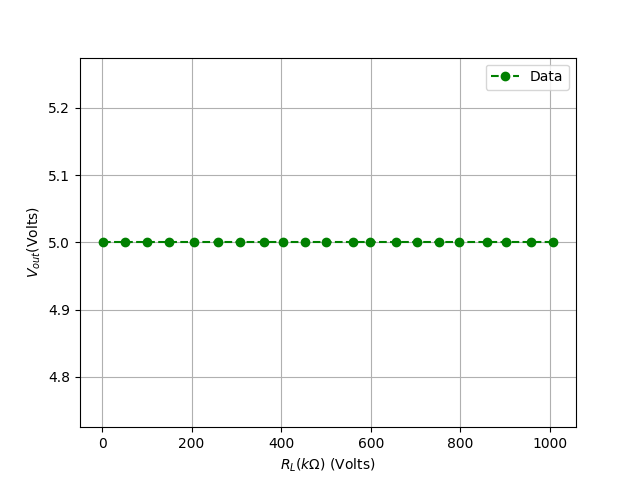
\includegraphics[width=0.9\textwidth]{D:/ronit/IISER-K/6 SEM/PH3204/Reports/exp01/part02_02.png} 
	\caption{Plot of $R_L$ v/s $V_{out}$}  
	\label{fig:part01_01}  
  \end{figure}
\section{Conclusion}
In this experiment we studied the voltage regulation property of zener diode. We determined the average breakdown volatge of the diode to be $5.63 $V, while on the second day (owing to a different zener diode), we found the breakdown voltage to be $6.54 V$ We also verified the fact that the voltage across the diode remained the same once we cross the breakdown voltage.\\
\\
Next we studied the voltage regulation property of IC 7805. We verfifed that the stable voltage of the IC is $5$V. We could also observe that the IC gave better regulation when compared to the zener diode.
\newpage
\section{Sources of Error}
The sources pf error in this experiment are as follows:
\begin{itemize}
	\item There can be inaccuracies in the measurement of the volatge and current using the multimeter. There may also be inaccuracies in the measurement of the resistance using the multimeter.
	\item The wires used in the experiment may not have negligible resistance. The same goes for the breadboard, the resistance of which may not be negligible.
\end{itemize}
\end{document}
